\section{Field-Effect Transistors}

Field-effect transistors (FETs) are three-terminal devices in which an electric
field controls the conductivity of a semiconductor channel. The gate electrode is
separated from the semiconductor by an insulating layer, so the gate voltage
modulates the channel charge without ideally causing a steady gate current. This
principle makes the FET a voltage-controlled device that can be used as a
switch, a variable resistor, or an amplifier. In an organic field-effect
transistor (OFET), the active channel is an organic semiconductor, and the mobile
charge carriers are usually confined to a thin accumulation layer near the
semiconductor--dielectric interface~\cite{Sirringhaus2005DevicePhysics,Bruetting2005}.

For this thesis, the FET is important in two related ways. First, it provides the
standard framework for describing gate-induced transport in organic thin films.
Second, the same electrostatic control of a sheet conductance is used in the
gated van der Pauw method discussed later. The following section therefore
summarizes the operating regimes, the ideal current--voltage relations, and the
small-signal concepts needed to interpret the measurements.

\subsection{Operation of Field-Effect Transistors}

A FET consists of a gate electrode, a gate dielectric, a semiconductor layer, and
two contacts called source and drain. The source is used as the reference
terminal. The gate--source voltage controls the density of mobile carriers in the
channel, while the drain--source voltage creates the lateral electric field that
drives these carriers. Thin-film transistors can be fabricated in several
geometries, for example as bottom-gate or top-gate and bottom-contact or
top-contact devices. These geometries affect injection and interface quality, but
the underlying field-effect mechanism remains the same
~\cite{Sirringhaus2005DevicePhysics,Natali2012ChargeInjection}.



\begin{figure}[htbp]
    \centering
    \begin{minipage}{0.48\textwidth}
        \centering
        \resizebox{\linewidth}{!}{

\begin{circuitikz}[scale=0.8]

% Device layout
\filldraw[black, fill = cyan!50, fill opacity = 0.3](-5,0)--(5,0)--(5,0.5)--(-5,0.5)--(-5,0);

\filldraw[black, fill = black!40, fill opacity = 0.5](-4,0.5)--(4,0.5)--(4,1)--(-4,1)--(-4,0.5);
\filldraw[black, fill=red!90, draw opacity=0.7](4,4)--(3,4)--(3,4.5)--(4,4.5)--(4,4);
\node at(0,0.75) []{G};

\filldraw[black, fill = blue!80, fill opacity=0.3](-4,1)--(4,1)--(4,2)--(-4,2)--(-4,1);

\filldraw[black, fill=green, fill opacity=0.5](-4,2)--(4,2)--(4,4)--(-4,4)--(-4,2);

\filldraw[black, fill=red!90, draw opacity=0.7](-4,4)--(-3,4)--(-3,4.5)--(-4,4.5)--(-4,4);
\node at(-3.5,4.25) []{S};
\filldraw[black, fill=red!90, draw opacity=0.7](4,4)--(3,4)--(3,4.5)--(4,4.5)--(4,4);
\node at(3.5,4.25) []{D};


% Wirings
\draw (-4,0.75)--(-6,0.75) to[vsource,l_=$V_\mathrm{GS}$] (-6,4.25)--(-4,4.25);
\draw (-3.5,4.5)--(-3.5,6) to[vsource,l_=$V_\mathrm{DS}$] (3.5,6)--(3.5,4.5);

% Channel
\draw[line width = 0.7pt, dashed, rounded corners=1ex] (-4,3)--(-3,3)--(-3,2.5)--(3,2.5)--(3,3)--(4,3);
\draw[line width = 0.7pt, dashed, rounded corners=1ex] (-4,3.5)--(-3,3.5)--(-3,4);
\draw[line width = 0.7pt, dashed, rounded corners=1ex] (4,3.5)--(3,3.5)--(3,4);


\newcommand{\holes}[2]
{
\shade [ball color=red] (#1,#2) circle (0.1);
}
\foreach \x in {-2.75,-2.25,...,2.75}{
  \foreach \y in {2.25}{
    \holes{\x}{\y}
  }
}
\foreach \x in {-3.75,-3.25}{
  \foreach \y in {2.25,2.75}{
    \holes{\x}{\y}
  }
}
\foreach \x in {3.75,3.25}{
  \foreach \y in {2.25,2.75}{
    \holes{\x}{\y}
  }
}
\foreach \x in {3.75,3.25,-3.75,-3.25}{
  \foreach \y in {3.75}{
    \holes{\x}{\y}
  }
}

\end{circuitikz}}\par
        \vspace{0.4em}
        Off/subthreshold: $V_\mathrm{GS} < V_\mathrm{T}$
    \end{minipage}\hfill
    \begin{minipage}{0.48\textwidth}
        \centering
        \resizebox{\linewidth}{!}{\input{figures/tikz/oFET-side-linear-1.tex}}\par
        \vspace{0.4em}
        Linear regime: $0<V_\mathrm{DS}\ll V_\mathrm{GS} - V_\mathrm{T}$
    \end{minipage}

    \vspace{1em}

    \begin{minipage}{0.48\textwidth}
        \centering
        \resizebox{\linewidth}{!}{

\begin{circuitikz}[scale=0.8]

% Device layout
\filldraw[black, fill = cyan!50, fill opacity = 0.3](-5,0)--(5,0)--(5,0.5)--(-5,0.5)--(-5,0);

\filldraw[black, fill = black!40, fill opacity = 0.5](-4,0.5)--(4,0.5)--(4,1)--(-4,1)--(-4,0.5);
\filldraw[black, fill=red!90, draw opacity=0.7](4,4)--(3,4)--(3,4.5)--(4,4.5)--(4,4);
\node at(0,0.75) []{G};

\filldraw[black, fill = blue!80, fill opacity=0.3](-4,1)--(4,1)--(4,2)--(-4,2)--(-4,1);

\filldraw[black, fill=green, fill opacity=0.5](-4,2)--(4,2)--(4,4)--(-4,4)--(-4,2);

\filldraw[black, fill=red!90, draw opacity=0.7](-4,4)--(-3,4)--(-3,4.5)--(-4,4.5)--(-4,4);
\node at(-3.5,4.25) []{S};
\filldraw[black, fill=red!90, draw opacity=0.7](4,4)--(3,4)--(3,4.5)--(4,4.5)--(4,4);
\node at(3.5,4.25) []{D};


% Wirings
\draw (-4,0.75)--(-6,0.75) to[vsource,l_=$V_\mathrm{GS}$] (-6,4.25)--(-4,4.25);
\draw (-3.5,4.5)--(-3.5,6) to[vsource,l_=$V_\mathrm{DS}$] (3.5,6)--(3.5,4.5);
\draw[->] (1,6)--++(1,0) node[above]{$I_\text{D}$};

% Channel
\draw[line width = 0.7pt, dashed, rounded corners=2ex] (-3,4)--(-3,3.25)--(3,2.5)--(3,4);

\newcommand{\holes}[2]
{
\shade [ball color=red] (#1,#2) circle (0.1);
}
\foreach \x in {-2.75,-2.25,...,2.75}{
  \foreach \y in {2.25}{
    \holes{\x}{\y}
  }
}
\foreach \x in {-2.75,-2.25, -1.75, -1.25}{
  \foreach \y in {2.75}{
    \holes{\x}{\y}
  }
}
\foreach \x in {-3.75,-3.25}{
  \foreach \y in {2.25,2.75, 3.25,3.75}{
    \holes{\x}{\y}
  }
}
\foreach \x in {3.75,3.25}{
  \foreach \y in {2.25,2.75, 3.25,3.75}{
    \holes{\x}{\y}
  }
}
% \holes{-3.5}{3.9};
% \holes{3.5}{3.9};
% \holes{-3.5}{2.5};
% \holes{3.5}{2.5};
% \draw[->](-3.5,3.8)--(-3.5,2.6);
% \draw[->](-3.4,2.5)--(3.4,2.5);
% \draw[->](3.5,2.6)--(3.5,3.8);

\end{circuitikz}}\par
        \vspace{0.4em}
        Linear regime: $0<V_\mathrm{DS}\lesssim V_\mathrm{GS} - V_\mathrm{T}$
    \end{minipage}\hfill
    \begin{minipage}{0.48\textwidth}
        \centering
        \resizebox{\linewidth}{!}{

\begin{circuitikz}[scale=0.8]

% Device layout
\filldraw[black, fill = cyan!50, fill opacity = 0.3](-5,0)--(5,0)--(5,0.5)--(-5,0.5)--(-5,0);

\filldraw[black, fill = black!40, fill opacity = 0.5](-4,0.5)--(4,0.5)--(4,1)--(-4,1)--(-4,0.5);
\filldraw[black, fill=red!90, draw opacity=0.7](4,4)--(3,4)--(3,4.5)--(4,4.5)--(4,4);
\node at(0,0.75) []{G};

\filldraw[black, fill = blue!80, fill opacity=0.3](-4,1)--(4,1)--(4,2)--(-4,2)--(-4,1);

\filldraw[black, fill=green, fill opacity=0.5](-4,2)--(4,2)--(4,4)--(-4,4)--(-4,2);

\filldraw[black, fill=red!90, draw opacity=0.7](-4,4)--(-3,4)--(-3,4.5)--(-4,4.5)--(-4,4);
\node at(-3.5,4.25) []{S};
\filldraw[black, fill=red!90, draw opacity=0.7](4,4)--(3,4)--(3,4.5)--(4,4.5)--(4,4);
\node at(3.5,4.25) []{D};


% Wirings
\draw (-4,0.75)--(-6,0.75) to[vsource,l_=$V_\mathrm{GS}$] (-6,4.25)--(-4,4.25);
\draw (-3.5,4.5)--(-3.5,6) to[vsource,l_=$V_\mathrm{DS}$] (3.5,6)--(3.5,4.5);
\draw[->] (1,6)--++(1,0) node[above]{$I_\text{D}$};

% Channel
\draw[line width = 0.7pt, dashed, rounded corners=2ex] (-3,4)--(-3,3.25)--(2,2);
\draw[line width = 0.7pt, dashed, rounded corners=1ex] (4,3)--(3,3)--(3,4);
\draw[->, red](1,2.5)--++(1.7,0.5);
\node[red, rotate=16.4, above = 3pt] at (1.85,2.55) {E-field};


\newcommand{\holes}[2]
{
\shade [ball color=red] (#1,#2) circle (0.1);
}
\foreach \x in {-2.75,-2.25,-1.75}{
  \foreach \y in {2.25,2.75}{
    \holes{\x}{\y}
  }
}
\foreach \x in {-1.25,-0.75,-0.25}{
  \foreach \y in {2.25}{
    \holes{\x}{\y}
  }
}
\foreach \x in {-3.75,-3.25}{
  \foreach \y in {2.25,2.75, 3.25,3.75}{
    \holes{\x}{\y}
  }
}
\foreach \x in {3.75,3.25}{
  \foreach \y in {3.25,3.75}{
    \holes{\x}{\y}
  }
}

\end{circuitikz}}\par
        \vspace{0.4em}
        Saturation: $V_\mathrm{DS}\geq V_\mathrm{GS} - V_\mathrm{T}$
    \end{minipage}
    \caption[Operating regimes of a $p$-channel field-effect transistor]{Schematic
    side views of the main operating regimes of a $p$-channel field-effect
    transistor. The voltage labels denote the positive bias magnitudes defined in
    Equation~\ref{eq:pfet_magnitude_convention}. Increasing gate bias forms a hole
    accumulation layer at the semiconductor--dielectric interface. Increasing
    drain bias makes the channel charge nonuniform and eventually produces
    pinch-off near the drain.}
    \label{fig:fet_operation_modes}
\end{figure}

The devices considered in this work are operated as $p$-channel transistors. A
gate voltage that is negative with respect to the source attracts holes to the
dielectric interface. A negative drain voltage then drives the accumulated holes
through the channel. To keep the notation compact, the following discussion uses
positive magnitudes for the relevant terminal quantities,
\begin{equation}
    V_\mathrm{GS}=\left|V_\mathrm{G}-V_\mathrm{S}\right|,
    \qquad
    V_\mathrm{DS}=\left|V_\mathrm{D}-V_\mathrm{S}\right|,
    \qquad
    I_\mathrm{D}=\left|I_\mathrm{D}\right|.
    \label{eq:pfet_magnitude_convention}
\end{equation}
The threshold voltage $V_\mathrm{T}$ is also written as a positive magnitude.
With this convention, the mathematical form of the equations is the same as for
an $n$-channel transistor, although the physical carriers are holes.

In the gradual-channel picture, the local channel potential is denoted by
$V(x)$, with $V(0)=0$ at the source and $V(L)=V_\mathrm{DS}$ at the drain. Above
threshold, the accumulated sheet charge is approximated by
\begin{equation}
    Q_\mathrm{p}(x)
    = C_\mathrm{i}\left[V_\mathrm{GS}-V_\mathrm{T}-V(x)\right],
    \label{eq:fet_local_sheet_charge}
\end{equation}
provided that the expression in brackets is positive. Here $C_\mathrm{i}$ is the
gate-insulator capacitance per unit area, and the two-dimensional hole density is
$p_\mathrm{2D}(x)=Q_\mathrm{p}(x)/q$. This relation shows why the channel is not
controlled by the gate voltage alone. At finite drain bias, the local potential
also changes along the channel, so the charge density can be nearly uniform at
small $V_\mathrm{DS}$ but strongly nonuniform at larger $V_\mathrm{DS}$
~\cite{Hu2010ModernSemiconductorDevices,Marinov2009OTFTPartI}.

The operating regimes in Figure~\ref{fig:fet_operation_modes} can then be
summarized as follows. Below threshold, only a small mobile charge density is
present and the device is nominally off. For $V_\mathrm{GS}>V_\mathrm{T}$ and
small $V_\mathrm{DS}$, a continuous accumulation channel connects source and
drain, and the transistor behaves approximately as a gate-controlled resistor.
When $V_\mathrm{DS}$ approaches $V_\mathrm{GS} - V_\mathrm{T}$, the channel charge near the drain
is reduced. At $V_\mathrm{DS}\geq V_\mathrm{GS} - V_\mathrm{T}$, the ideal model predicts
pinch-off at the drain side and the current enters the saturation regime.

The threshold voltage should not be understood as a sharp microscopic boundary
between an empty and a conducting channel. It is an effective device parameter
that includes the flat-band condition, localized states, fixed dielectric charge,
mobile ions, and trapped charge. These contributions can shift
$V_\mathrm{T}$ and can cause hysteresis between forward and backward gate-voltage
sweeps. Such effects are especially relevant in OFETs, where the density of
localized states is often broad~\cite{Bruetting2005,Sirringhaus2005DevicePhysics}.

\subsection{Current--Voltage Relationship}

The standard current--voltage relations are obtained within the gradual-channel
approximation. The model assumes a long and laterally uniform channel, a constant
mobility $\mu$, a uniform gate capacitance, negligible gate leakage, and no
voltage loss at the source and drain contacts. The drift current at position $x$
is written as
\begin{equation}
    I_\mathrm{D}
    = W\mu Q_\mathrm{p}(x)\frac{\mathrm{d}V}{\mathrm{d}x},
    \label{eq:fet_local_current}
\end{equation}
where $W$ and $L$ are the channel width and length. Substitution of
Equation~\ref{eq:fet_local_sheet_charge} and integration from source to drain
gives
\begin{equation}
    I_\mathrm{D}
    = \mu C_\mathrm{i}\frac{W}{L}
    \left[
        \left(V_\mathrm{GS}-V_\mathrm{T}\right)V_\mathrm{DS}
        -\frac{V_\mathrm{DS}^{2}}{2}
    \right],
    \qquad
    0\leq V_\mathrm{DS}<V_\mathrm{GS} - V_\mathrm{T}.
    \label{eq:fet_linear_current}
\end{equation}
This expression describes the linear regime. At small drain bias, the quadratic
term is negligible and
\begin{equation}
    I_\mathrm{D}
    \approx \mu C_\mathrm{i}\frac{W}{L}
    \left(V_\mathrm{GS}-V_\mathrm{T}\right)V_\mathrm{DS}.
    \label{eq:fet_low_vds_current}
\end{equation}
The channel conductance is then proportional to the gate overdrive, which is the
basis for viewing the FET as a voltage-controlled resistor.

At the onset of pinch-off, $V_\mathrm{DS}=V_\mathrm{GS} - V_\mathrm{T}$. Inserting this condition
into Equation~\ref{eq:fet_linear_current} yields the ideal saturation current
\begin{equation}
    I_\mathrm{D,sat}
    = \frac{1}{2}\mu C_\mathrm{i}\frac{W}{L}
    \left(V_\mathrm{GS}-V_\mathrm{T}\right)^2,
    \qquad
    V_\mathrm{DS}\geq V_\mathrm{GS} - V_\mathrm{T}.
    \label{eq:fet_saturation_current}
\end{equation}
In the ideal model, the saturation current is independent of drain voltage. Real
output curves usually retain a finite slope because of channel-length modulation,
field-dependent mobility, contact effects, or changes in trap occupation during
the measurement. This nonideality is often represented phenomenologically by
\begin{equation}
    I_\mathrm{D,sat}
    \approx \frac{1}{2}\mu C_\mathrm{i}\frac{W}{L}
    \left(V_\mathrm{GS}-V_\mathrm{T}\right)^2
    \left(1+\lambda V_\mathrm{DS}\right),
    \label{eq:fet_channel_length_modulation}
\end{equation}
where $\lambda$ is the channel-length-modulation parameter.

Experimentally, FETs are commonly described by transfer and output
characteristics. A transfer curve records $I_\mathrm{D}$ as a function of
$V_\mathrm{GS}$ at fixed drain bias and is used to estimate the threshold
voltage, on/off ratio, subthreshold behavior, and apparent mobility. An output
curve records $I_\mathrm{D}$ as a function of $V_\mathrm{DS}$ for different gate
voltages and shows the transition from the linear regime to saturation. The same
plots can also reveal injection limitations, for example nonlinear or S-shaped
curves near the origin~\cite{Natali2012ChargeInjection,Marinov2009OTFTPartI}.

\begin{figure}[htbp]
    \centering
    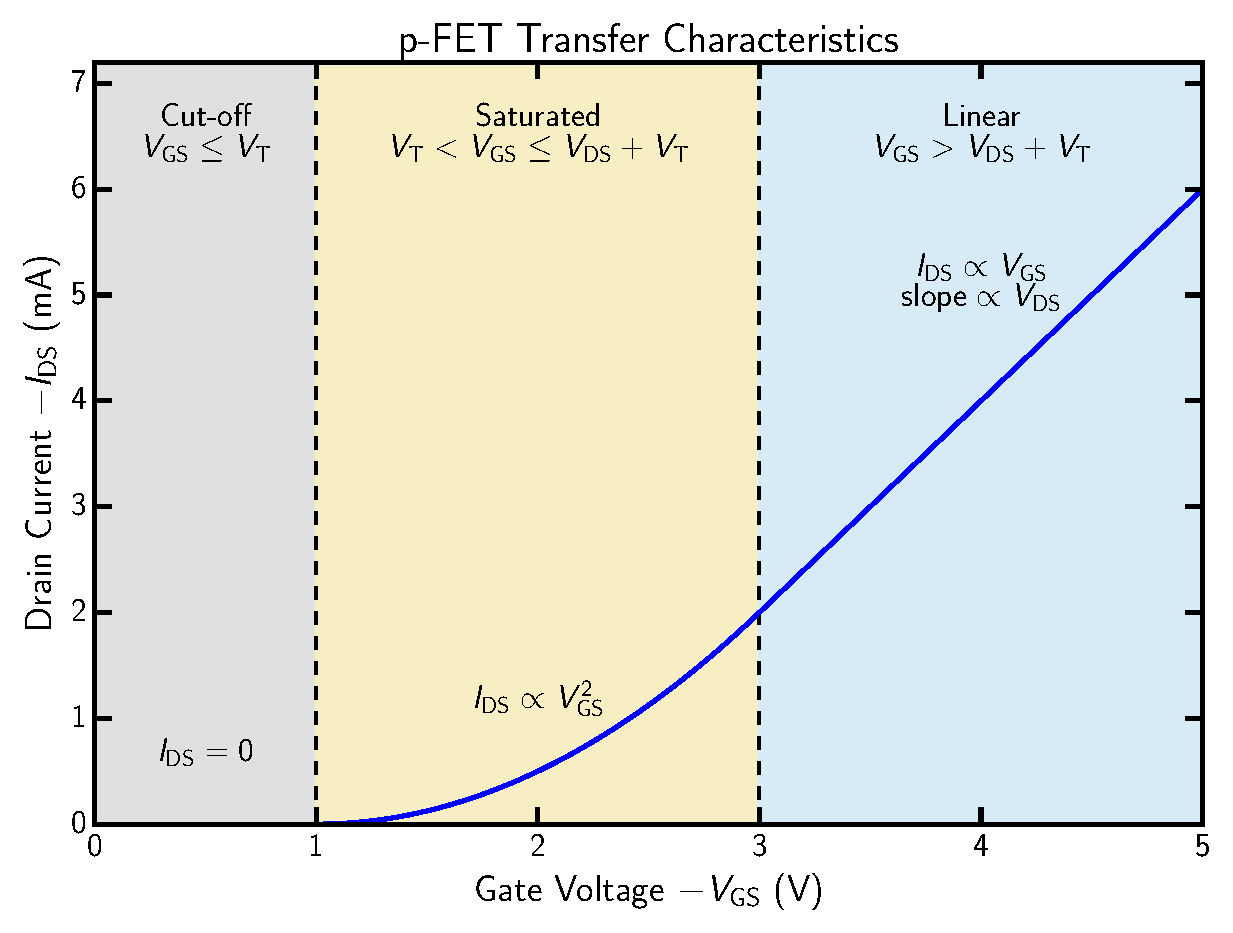
\includegraphics[width=0.495\textwidth]{figures/Transfer}
    \hfill
    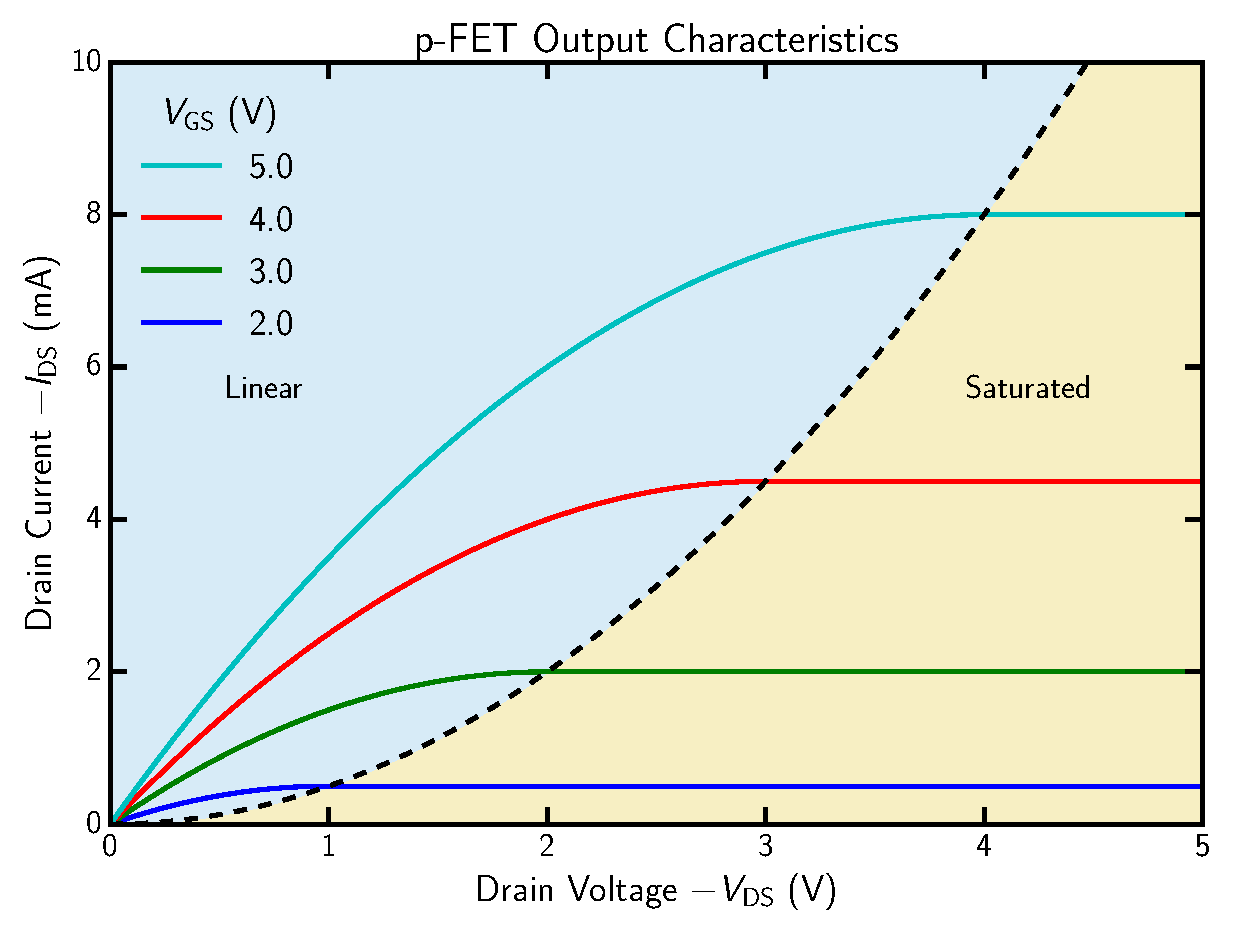
\includegraphics[width=0.495\textwidth]{figures/Output}
    \caption[Idealized transfer and output characteristics of a $p$-channel FET]{Idealized
    transfer characteristic at fixed drain bias (left) and output characteristics
    at several gate voltages (right). For consistency with
    Equation~\ref{eq:pfet_magnitude_convention}, the axes show the magnitudes of
    the $p$-channel voltages and current. In the linear regime,
    $I_\mathrm{D}$ is approximately linear in gate overdrive and drain voltage.
    In saturation, $I_\mathrm{D}$ is approximately quadratic in gate overdrive
    and ideally independent of drain voltage.}
    \label{fig:fet_transfer_output_characteristics}
\end{figure}

For a small and constant drain bias, Equation~\ref{eq:fet_low_vds_current} gives
the linear-regime mobility
\begin{equation}
    \mu_\mathrm{lin}
    = \frac{L}{W C_\mathrm{i}V_\mathrm{DS}}
    \frac{\mathrm{d}I_\mathrm{D}}{\mathrm{d}V_\mathrm{GS}}.
    \label{eq:fet_linear_mobility}
\end{equation}
In saturation, Equation~\ref{eq:fet_saturation_current} predicts a linear
relation between $\sqrt{I_\mathrm{D}}$ and $V_\mathrm{GS}$. The corresponding
mobility estimate is
\begin{equation}
    \mu_\mathrm{sat}
    = \frac{2L}{W C_\mathrm{i}}
    \left(
        \frac{\mathrm{d}\sqrt{I_\mathrm{D}}}
        {\mathrm{d}V_\mathrm{GS}}
    \right)^2.
    \label{eq:fet_saturation_mobility}
\end{equation}
These values are model-dependent. If the mobility depends on carrier density,
electric field, or contact injection, the extracted mobility is an apparent or
differential quantity rather than a unique material constant.

Contact resistance is a major limitation in thin-film transistors. The measured
terminal voltage is divided between the channel and the contacts,
\begin{equation}
    R_\mathrm{tot}=R_\mathrm{C}+R_\mathrm{ch}.
    \label{eq:fet_total_resistance}
\end{equation}
A large $R_\mathrm{C}$ could change the internal channel voltage and
can distort the slope of the transfer curve. In OFETs, this can lead to mobility
peaks or to a significant overestimation of the channel mobility
~\cite{Bittle2016MobilityOverestimation,Natali2012ChargeInjection}. This is one
reason why the contact-independent gated van der Pauw method, introduced in
Section~\ref{sec:gated_van_der_pauw_method}, is useful for the present work
~\cite{Rolin2017GVDP}.

\subsection{Small-Signal Amplification Properties}

Besides switching, a FET can amplify small voltage variations. In a switching
application, the transistor is driven between a high-resistance off state and a
low-resistance on state. In an amplifier, by contrast, the device is held at a
stationary operating point and only small perturbations around this point are
used. The gate-voltage variation then modulates the channel current, and a load
resistor converts this current variation into an output-voltage variation.
Figure~\ref{fig:fet_switch} first illustrates the corresponding switching
principle for a simple resistive-load circuit.

\begin{figure}[htbp]
    \centering
    \resizebox{0.35\textwidth}{!}{\begin{circuitikz}[scale=0.5]
\ctikzset{resistor = european}
\ctikzset{tripoles/mos style/arrows}
\draw
(0,0)     node[nmos] (nmos){}
(nmos.G) node[above] {G}
    to[short] ++(-3,0)

(nmos.S) node[left] {S}
    to[R,l=$R_\text{S}$] ++(0,-4.5) node[rground]{}
(nmos.D) node[left] {D}
    to[short]++(0,1) to[R,l_=$R_\text{D}$]++(0,3);
\draw[->,red](0,5.5) -- ++(0,1) node[right]{$V_\text{DD}$};
\draw[](-5,-6)--(5,-6);
\draw (-5,-6) to[short,-*](0,-6);
\draw (nmos.D) to[short,*-] ++(5,0);

\draw[->,red] (-5,-5.9)--(-5,-0.1);
\node at(-5,-3) [left]{\color{red}$V_\text{in}$};
 \draw[->,blue] (5,-5.9)--(5,1.5-0.1);
 \node at(5,-2.25) [right]{\color{blue}$V_\text{out}$};

\end{circuitikz}}
    \caption[FET used as a voltage-controlled switch]{FET used as a
    voltage-controlled switch in a resistive circuit. A change of gate voltage
    changes the channel resistance and therefore the output voltage at the drain.
    The schematic uses the conventional $n$-channel polarity; a $p$-channel
    implementation requires reversed polarities.}
    \label{fig:fet_switch}
\end{figure}

At an operating point $Q$, the terminal quantities are written as a DC bias plus
a small time-dependent signal,
\begin{equation}
    V_\mathrm{GS}(t)=V_\mathrm{GS,Q}+v_\mathrm{gs}(t),
    \qquad
    V_\mathrm{DS}(t)=V_\mathrm{DS,Q}+v_\mathrm{ds}(t),
    \qquad
    I_\mathrm{D}(t)=I_\mathrm{D,Q}+i_\mathrm{d}(t).
    \label{eq:fet_small_signal_decomposition}
\end{equation}
Linearization of the current--voltage relation gives
\begin{equation}
    i_\mathrm{d}
    = g_\mathrm{m}v_\mathrm{gs}+g_\mathrm{ds}v_\mathrm{ds},
    \label{eq:fet_small_signal_current}
\end{equation}
where
\begin{equation}
    g_\mathrm{m}
    = \left.\frac{\partial I_\mathrm{D}}{\partial V_\mathrm{GS}}
      \right|_{V_\mathrm{DS}}
    \label{eq:fet_transconductance_definition}
\end{equation}
is the transconductance and
\begin{equation}
    g_\mathrm{ds}
    = \left.\frac{\partial I_\mathrm{D}}{\partial V_\mathrm{DS}}
      \right|_{V_\mathrm{GS}},
    \qquad
    r_\mathrm{o}=\frac{1}{g_\mathrm{ds}}
    \label{eq:fet_output_conductance}
\end{equation}
is the output conductance, with $r_\mathrm{o}$ the corresponding output
resistance. The transconductance converts an input-voltage variation into a
current variation, while the output resistance describes the finite slope of the
output curve in saturation.

Using the ideal saturation expression, the transconductance becomes
\begin{equation}
    g_\mathrm{m}(V_\mathrm{GS,Q})
    = \mu C_\mathrm{i}\frac{W}{L}
      \left(V_\mathrm{GS,Q}-V_\mathrm{T}\right).
    \label{eq:fet_gm_saturation}
\end{equation}
Thus, the small-signal response increases with mobility, gate capacitance,
width-to-length ratio, and bias current. In the ideal saturation model,
$g_\mathrm{ds}=0$ and $r_\mathrm{o}$ is infinite. With channel-length modulation,
$r_\mathrm{o}\approx 1/(\lambda I_\mathrm{D,Q})$.

Figure~\ref{fig:fet_common_source_amplifier} shows a common-source amplifier,
which is the circuit principle used later for the OFET amplification
measurement. The resistors $R_1$ and $R_2$ set the gate bias, $R_\mathrm{D}$
converts drain-current variations into an output voltage, and $R_\mathrm{S}$
stabilizes the operating point. The input and output coupling capacitors separate
the DC bias from neighboring circuits, while the source-bypass capacitor can
short-circuit $R_\mathrm{S}$ for the AC signal. The schematic is drawn with the
usual $n$-channel polarity. For the $p$-channel OFETs investigated in this work,
the physical supply and terminal polarities are reversed, but the small-signal
relations have the same form when the positive voltage magnitudes of
Equation~\ref{eq:pfet_magnitude_convention} are used.

If the source-bypass capacitor acts as a short circuit for the signal frequency,
the mid-band voltage gain is approximately
\begin{equation}
    A_\mathrm{v}
    = \frac{v_\mathrm{out}}{v_\mathrm{in}}
    \approx -g_\mathrm{m}
    \left(R_\mathrm{D}\parallel r_\mathrm{o}\parallel R_\mathrm{L}\right).
    \label{eq:fet_common_source_gain}
\end{equation}
The minus sign denotes phase inversion between gate input and drain output. If
$R_\mathrm{S}$ is not bypassed, source degeneration reduces the gain approximately
to
\begin{equation}
    A_\mathrm{v}
    \approx
    -\frac{g_\mathrm{m}
    \left(R_\mathrm{D}\parallel r_\mathrm{o}\parallel R_\mathrm{L}\right)}
    {1+g_\mathrm{m}R_\mathrm{S}},
    \label{eq:fet_source_degenerated_gain}
\end{equation}
but improves bias stability and linearity. In practice the effective load also
contains the finite input resistance of the measuring instrument or following
circuit. Because the gate is insulated, the low-frequency input resistance of an
ideal FET is very high, so the gate-bias network mainly determines the input
resistance of the amplifier stage.

\begin{figure}[htbp]
    \centering
    \resizebox{0.62\textwidth}{!}{\begin{circuitikz}[scale=0.5]
\ctikzset{resistor = european}
\ctikzset{tripoles/mos style/arrows}
\draw
(0,0)     node[nmos] (nmos){}
(nmos.G) node[above] {G}
    to[short] ++(-3,0)

(nmos.S) node[left] {S}
    to[R,l=$R_\text{S}$] ++(0,-4.5) node[rground]{}
(nmos.D) node[left] {D}
    to[short]++(0,1) to[vR,l_=$R_\text{D}$]++(0,3);
\draw[->,red](0,5.5) -- ++(0,2) node[right]{$V_\text{DD}$};
\draw[](6,-6)--(-5,-6) to[R,l_=$R_2$,*-*] (-5,0) to[vR,l_=$R_1$] (-5,6)to[short,-*](0,6);
\draw (-10,-6) to[short,-*](0,-6);
\draw (nmos.D) to[C,l_=$C_o$,*-] ++(6,0);

\draw (-5,0) to[C,l_=$C_i$,*-] (-10,0);

\draw[red] (nmos.S) to[short,*-]++(3,0)to[C,l = $C_\text{S}$,-*] ++(0,-4.5);


\draw[blue, line width = 0.5mm,smooth,domain=7:9.5,samples=200] plot (\x,{-1*sin(360*(\x+8)*1)+1.5});
\draw[red,dashed, line width = 0.3mm,smooth,domain=7:9.5,samples=200] plot (\x,{0.25*sin(360*(\x+8)*1)+1.5});
\draw[->](6.5,1.5)--(10,1.5)node[below]{$t$};

\draw[red, line width = 0.5mm,smooth,domain=-14:-11.5,samples=200] plot (\x,{0.25*sin(360*(\x-11)*1)});
\draw[->](-14.5,0)--(-11,0)node[below]{$t$};

\draw[->,red] (-10,-5.9)--(-10,-0.1);
\node at(-10,-3) [left]{\color{red}$V_\text{in}$};
 \draw[->,blue] (6,-5.9)--(6,1.5-0.1);
 \node at(6,-2.25) [right]{\color{blue}$V_\text{out} = A(V_\text{G})\cdot V_\text{in}$};
\end{circuitikz}}
    \caption[Common-source FET amplifier]{Common-source FET amplifier with a
    resistive drain load, gate-bias network, source stabilization, and coupling
    capacitors. The source-bypass capacitor increases the AC gain by suppressing
    source degeneration over its effective frequency range. The output signal is
    amplified and inverted relative to the input signal.}
    \label{fig:fet_common_source_amplifier}
\end{figure}

The useful bias point for voltage amplification lies where the static amplifier
transfer curve has a sufficiently steep and approximately linear slope, while the
output voltage still has headroom for both positive and negative signal swings.
Locally, the measured voltage gain is the slope
\begin{equation}
    A_\mathrm{v}(Q)
    = \left.\frac{\partial V_\mathrm{out}}{\partial V_\mathrm{in}}
      \right|_{Q}.
    \label{eq:fet_static_gain_slope}
\end{equation}
This is illustrated in Figure~\ref{fig:fet_amplifier_transfer_gain}. Biasing too
close to cut-off gives a small transconductance, whereas biasing too far into the
strongly conducting regime leaves little output-voltage headroom and can reduce
the small-signal gain. A large input signal moves the device over a curved part
of the transfer characteristic and therefore causes nonlinear distortion. A
larger $R_\mathrm{D}$ usually increases the magnitude of the gain, but it also
narrows the useful bias range and increases the RC time constants of the circuit.

\begin{figure}[htbp]
    \centering
    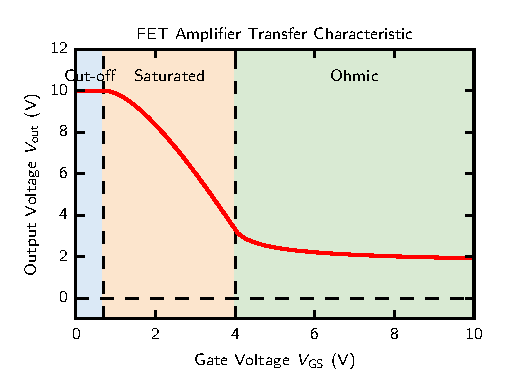
\includegraphics[width=0.48\textwidth]{figures/theo-amp-transfer}
    \hfill
    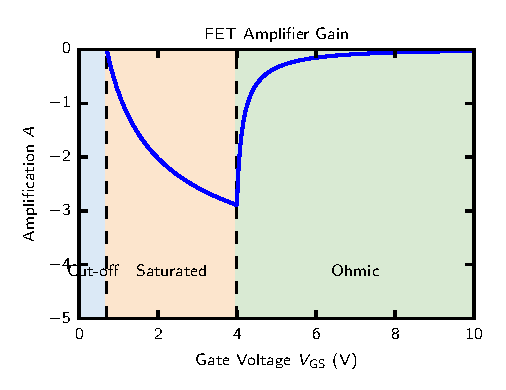
\includegraphics[width=0.48\textwidth]{figures/theo-amp-gain}
    \caption[FET amplifier transfer characteristic and small-signal gain]{FET amplifier transfer characteristic and small-signal gain. The left panel shows the static output
    voltage as a function of gate bias. The local slope of this curve determines
    the voltage gain shown on the right. The gain is negative in the inverting
    common-source configuration and is largest in magnitude within the transition
    region between cut-off and strongly ohmic operation.}
    \label{fig:fet_amplifier_transfer_gain}
\end{figure}


